%!TEX root = ../skripsi.tex
%-------------------------------------------------------------------------------
%                            BAB III
%               		METODOLOGI PENELITIAN
%-------------------------------------------------------------------------------
\begin{spacing}{2}
\chapter{METODE PENGEMBANGAN SISTEM}

  Penelitian ini dibuat untuk menganalisis konsep implementasi aplikasi berita berbasis \emph{mobile}, sehingga aplikasi dapat berjalan dengan efektif dan efisien. Sebelum penelitian ini dilakukan riset terlebih dahulu untuk menjaring data serta informasi terkait. Tahap pengumpulan data pada penelitian ini dilakukan dengan metode observasi.

  Kegiatan pengumpulan data secara observasi dilakukan dengan mencoba langsung aplikasi sejenis. Selain itu peneliti juga mengamati fitur dan tata letak dari aplikasi sejenis. Kegiatan observasi dilakukan untuk mengetahui fitur dan keunggulan dari aplikasi sejenis lainnya. Kegiatan observasi dilakukan pada aplikasi \emph{mobile} milik NYTimes, Kompas, dan Detikcom.

  Dalam penelitian ini, metode pengembangan sistem yang digunakan adalah \emph{extreme programming} dengan menggunakan praktek pengembangan \emph{test driven development} dan \emph{tools} UML untuk menggambarkan diagram \emph{use case}. Pemilihan metode ini dikarenakan aplikasi yang dikembangkan berfokus pada \emph{coding} dan \emph{testing} yang mencoba meningkatkan efisiensi dan fleksibilitas dari sebuah proyek pengembangan perangkat lunak. Tahapan metode pengembangan sistem terbagi menjadi 4 tahapan, yaitu \emph{exploration}, \emph{planning}, \emph{iterations}, dan \emph{productionizing}.

  \section{Tahap \emph{Exploration}}
    Pada tahapan ini, terdapat beberapa kegiatan yang dilakukan dalam membangun sebuah aplikasi berita berbasis \emph{mobile}, antara lain:

    \subsection{Identifikasi Ruang Lingkup dan Kebutuhan Sistem}
      Pada tahap ini peneliti mengidentifikasi ruang lingkup dan kebutuhan aplikasi berita berbasis \emph{mobile}, peneliti melakukan observasi terlebih dahulu pada aplikasi sejenis yang sudah ada sebelumnya untuk mengetahui ruang lingkup aplikasi kemudian menganalisis kebutuhan pengguna terhadap aplikasi \emph{mobile} yang akan dibangun. Identifikasi ruang lingkup dan kebutuhan pengguna menghasilkan \emph{user story}.

    \subsection{Menentukan Tools dan Teknologi}
      Pada tahap ini peneliti menentukan \emph{tools} dan teknologi yang dibutuhkan untuk membangun aplikasi berita berbasis \emph{mobile}. Peneliti dapat mengetahui \emph{tools} dan teknologi apa saja yang dibutuhkan berdasarkan hasil identifikasi dan kebutuhan ruang lingkup yang telah dilakukan sebelumnya. \emph{Tools} dan teknologi tersebut berupa bahasa pemgrograman, kerangka kerja, pustaka serta perangkat lunak lainnya yang mendukung pengembangan aplikasi berita berbasis \emph{mobile}.

  \section{Tahap \emph{Planning}}
    Pada tahapan \emph{planning} ada beberapa langkah yang dilakukan dalam membangun sebuah aplikasi berita berbasis \emph{mobile}.

    \subsection{Menentukan Batasan dan Prioritas}
      Pada tahap ini peneliti menentukan batasan dan prioritas berdasarkan identifikasi ruang lingkup yang telah dibuat pada tahap sebelumnya untuk merancang batasan dan prioritas pada masing-masing \emph{user story}. Sehingga ruang lingkup dipecah menjadi beberapa \emph{user story} yang mewakili perangcangan fitur-fitur dari fungsi aplikasi \emph{mobile}.

    \subsection{Membuat Rencana Peluncuran}
      Pada tahap ini peneliti membuat rencana peluncuran untuk merancang ada berapa kali iterasi yang nantinya akan terjadi dalam membangun aplikasi \emph{mobile}. Perancangan iterasi akan terus berulang sesuai dengan kebutuhan \emph{client} yang dituangkan dalam \emph{user story}.

    \subsection{Menyiapkan Uji Penerimaan Pengguna}
      Pada tahap ini peneliti menyiapkan metode apa yang nantinya aplikasi yang dibangun akan di uji, seperti apa proses pengujiannya, dan fitur apa saja yang nantinya akan diuji agar mencapai hasil sesuai dengan kebutuhan aplikasi.

  \section{Tahap \emph{Iterations}}
    Pada tahapan \emph{iterations} dilakukan perulangan selama beberapa kali sesuai dengan lolos atau tidaknya hasil uji untuk mendapatkan hasil yang sesuai dengan keinginan pengguna. Perulangan tersebut dilakukan sesuai dengan \emph{user story} yang telah dibuat pada tahap sebelumnya. Serta tahap pembersihan atau \emph{refactoring} yang berguna untuk memastikan kelayakan dari implementasi. Berikut bagan alur proses dari pengembangan.

    \begin{figure}[H]
      \centering
      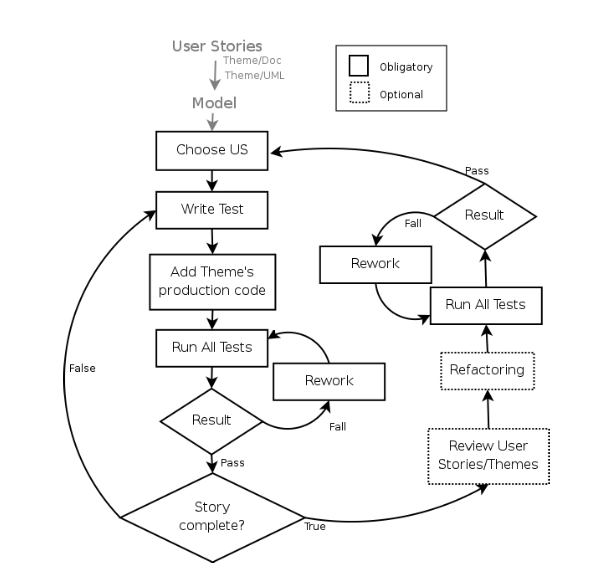
\includegraphics[width=1\textwidth]{images/bagan-tdd}
      \caption{Bagan Alur \emph{Test Driven Development}}
      \label{bagan-tdd}
    \end{figure}

    \subsection{Penambahan Tes}
      Pada tahap ini peneliti menulis kode tes baru untuk semua fitur baru yang akan dikembangkan atau menyesuaikan tes sebelumnya. Tes dibuat berdasarkan dari \emph{user story} untuk memenuhi kebutuhan dan menghindari kebutuhan diluar batasan.

    \subsection{Menjalankan Tes Dan Melihat Tes Yang Gagal}
      Pada tahap ini peneliti melakukan pengujian dengan menjalankan semua tes yang telah ditulis, dan melihat tes yang tidak lolos untuk menulis implementasi dari \emph{behavior} yang belum diimplementasikan. Tes yang ditambahkan untuk fitur baru seharusnya tidak lolos pada tahap ini.

    \subsection{Implementasi}
      Pada tahap ini peneliti melakukan implementasi fitur pada aplikasi berdasarkan hasil tes yang tidak lolos uji.

    \subsection{Menjalankan Tes}
      Pada tahap ini peneliti melakukan pengujian setelah implementasi disesuaikan dengan hasil tes sebelumnya. Jika hasil tes lolos uji, maka fitur tersebut sudah sesuai dengan kebutuhan berdasarkan tes yang telah dilewati. Jika hasil tes tidak lolos uji, maka proses akan berulang kembali ke tahap implementasi.

    \subsection{\emph{Refactoring}}
      Pada tahap ini peneliti melakukan pembersihan terhadap kode setelah beberapa kali proses implementasi dan pengujian. Menghapus duplikasi yang terjadi pada implementasi \emph{Object}, \emph{Class}, \emph{Module}, dan \emph{Method} karena harus mempresentasikan tujuan dan penggunaannya, selagi fungsionalitas mereka ditambahkan. Tahap ini berguna untuk mempertajam \emph{readability} dan \emph{maintainability} yang mana dapat menambahkan nilai dalam \emph{lifecyle}.

  \section{Tahap \emph{Productionizing}}
    Pada tahap ini dilakukan pengujian dari aplikasi \emph{mobile}. Pengujian dilakukan dengan cara simulasi aplikasi versi \emph{debug} pada perangkat \emph{mobile} atau \emph{Simulator} perangkat \emph{mobile}.

\section{Kebutuhan Pengembangan Sistem}
	Pengembangan aplikasi berbasis \emph{mobile} membutuhkan perangkat lunak menulis kode aplikasi dan perangkat keras untuk menjalankannya.

	\subsection{Perangkat Keras}
		Spesifikasi perangkat keras yang dibutuhkan untuk mengembangkan aplikasi adalah sebagai berikut:

		\vspace{-0.5cm}

		\begin{enumerate}[a.]
		\itemsep0em
			\item Macbook Air 13"
			\item Memory 4 GB
			\item Harddisk 256 GB
			\item HP Android
			\item iPhone 6
		\end{enumerate}

	\subsection{Perangkat Lunak}
		Perangkat lunak yang dibutuhkan untuk mengembangkan aplikasi adalah sebagai berikut:

		\vspace{-0.5cm}

		\begin{enumerate}[a.]
		\itemsep0em
			\item Sublime Text 3
			\item NodeJS
			\item Reactroton
			\item Web Browser
			\item Git dan Akun Github.com
			\item Akun Travis-CI.com
		\end{enumerate}

\section{Jadwal Penelitian}
	\begin{table}[H]
  \centering
  \caption{Jadwal Penelitian}
  \label{my-label}
  \begin{tabular}{|c|l|l|l|l|l|l|l|l|l|l|l|l|l|}
  \hline
                                & \multicolumn{1}{c|}{}                                    & \multicolumn{12}{c|}{\textbf{Bulan}}                                                                                                                                                             \\ \cline{3-14} 
                                & \multicolumn{1}{c|}{}                                    & \multicolumn{4}{c|}{Oktober}                                                         & \multicolumn{4}{c|}{November}                             & \multicolumn{4}{c|}{Desember}                 \\ \cline{3-14} 
  \multirow{-3}{*}{\textbf{No}} & \multicolumn{1}{c|}{\multirow{-3}{*}{\textbf{Kegiatan}}} & 1                     & 2                             & 3             & 4            & 1        & 2        & 3        & 4                        & 1         & 2         & 3         & 4         \\ \hline
  1                             & Seminar Proposal                                         & \multicolumn{2}{l|}{\cellcolor[HTML]{656565}}         &               &              &          &          &          &                          &           &           &           &           \\ \hline
  2                             & Exploration dan Planning                                 &                       & \multicolumn{2}{l|}{\cellcolor[HTML]{656565}} &              &          &          &          &                          &           &           &           &           \\ \hline
  3                             & Iterations                                               &                       &                               &               & \multicolumn{4}{l|}{\cellcolor[HTML]{656565}} &                          &           &           &           &           \\ \hline
  4                             & Productionizing                                          &                       &                               &               &              &          &          &          & \cellcolor[HTML]{656565} &           &           &           &           \\ \hline
  5                             & Penyelesaian Laporan                                     &                       &                               &               &              &          &          &          &                          & \multicolumn{4}{l|}{\cellcolor[HTML]{656565}} \\ \hline
  \end{tabular}
  \end{table}

\end{spacing}
% Baris ini digunakan untuk membantu dalam melakukan sitasi
% Karena diapit dengan comment, maka baris ini akan diabaikan
% oleh compiler LaTeX.
\begin{comment}
\bibliography{daftar-pustaka}
\end{comment}
